% Group Number 31 -- Human or AI? Kaggle report (course template, filled in).
% Self-contained: upload only this file to Overleaf. Blocks between "% <<gen ..." and "% gen>>" are copied from
% the repository's generated results by reports/inline_tables.py; do not edit them by hand.
\documentclass[11pt,letterpaper]{article}
\usepackage[margin=0.86in]{geometry}
\usepackage[T1]{fontenc}
\usepackage[utf8]{inputenc}
\usepackage{lmodern}
\usepackage{xcolor}
\usepackage{tabularx,booktabs,array,longtable}
\usepackage{enumitem}
\usepackage{hyperref}
\usepackage{fancyhdr}
\usepackage{lastpage}
\usepackage{titlesec}
\usepackage{amsmath,amssymb}
\usepackage{microtype}
\usepackage{needspace}
\usepackage{ragged2e}
\usepackage{pgfplots}
\pgfplotsset{compat=1.18}
\definecolor{navy}{HTML}{19334C}
\definecolor{teal}{HTML}{236B82}
\definecolor{soft}{HTML}{EFF5F7}
\definecolor{muted}{HTML}{52616B}
\definecolor{copper}{HTML}{C0763A}
\hypersetup{colorlinks=true,linkcolor=teal,urlcolor=teal,citecolor=teal}
\titleformat{\section}{\Large\bfseries\color{navy}}{\thesection.}{0.6em}{}
\titleformat{\subsection}{\large\bfseries\color{navy}}{\thesubsection}{0.6em}{}
\titleformat{\subsubsection}{\normalsize\bfseries\color{navy}}{\thesubsubsection}{0.6em}{}
\titlespacing*{\section}{0pt}{15pt}{6pt}
\titlespacing*{\subsection}{0pt}{10pt}{4pt}
\setlength{\parindent}{0pt}
\setlength{\parskip}{4.5pt}
\setlength{\headheight}{15pt}
\renewcommand{\arraystretch}{1.16}
\setlist[itemize]{topsep=3pt,itemsep=2pt,leftmargin=1.4em}
\setlist[enumerate]{topsep=3pt,itemsep=2pt,leftmargin=1.5em}
\pagestyle{fancy}
\fancyhf{}
\fancyhead[L]{\small\color{muted} Applied Machine Learning \textbar{} Cornell Tech}
\fancyhead[R]{\small\color{muted} Human or AI?}
\fancyfoot[C]{\small\color{muted} Page \thepage\ of \pageref{LastPage}}
\renewcommand{\headrulewidth}{0.3pt}
\newcommand{\placeholder}[1]{\par\noindent\textcolor{teal}{\textit{[Your response: #1]}}\par\vspace{0.3em}}
\newcommand{\figplaceholder}[1]{\par\noindent\fcolorbox{teal}{soft}{\parbox[c][1.15in][c]{0.94\linewidth}{\centering\textcolor{muted}{Insert #1 here}}}\par}
\newcommand{\question}[2]{\needspace{4\baselineskip}\par\addvspace{0.45em}\noindent\textbf{#1}\quad #2\par\nobreak\vspace{0.1em}}
\newcommand{\smallnote}[1]{{\small\color{muted}#1}}
\newcolumntype{Y}{>{\RaggedRight\arraybackslash}X}
\newcommand{\commit}[2]{\href{https://github.com/ZhenmanShen/human-or-ai-submissions/commit/#1}{\texttt{#2}}}
\expandafter\def\expandafter\UrlBreaks\expandafter{\UrlBreaks\do\-\do\.}
\newcommand{\hf}[1]{{\small\nolinkurl{#1}}}% Hugging Face ids; may break at / - .
\begin{document}
\thispagestyle{empty}
\vspace*{0.2in}
{\color{teal}\bfseries CORNELL TECH \textbar{} APPLIED MACHINE LEARNING}\par
\vspace{0.15in}
{\Huge\bfseries\color{navy} Human or AI?}\par
\vspace{0.07in}
{\LARGE\color{navy} Kaggle Competition Report --- Group Number 31}\par
\vspace{0.17in}

\textbf{Report Template: }\href{https://www.overleaf.com/project/6ae1fc85355dcf680137d898/share#f2777b20d3adeeecfac9096f78008e2f8daa0ff4be43de3b}{TEMPLATE}

\textbf{Github Repository Template: }\href{https://github.com/sekhari/human-or-ai-submissions}{REPO}

\textbf{Welcome to the competition!} Your task is to build a machine learning classifier that predicts whether a passage was written by a human or generated by an AI model. You will use a labeled training set, an additional unlabeled set, and a held-out Kaggle test set. The aim is not just a high leaderboard score: we want you to compare methods, design careful experiments, understand generalization, and explain what your results actually show.

You are encouraged to try several approaches. A well-tested logistic regression or support vector machine is just as legitimate as a neural network. The project is designed to be approachable on a laptop; a GPU is \emph{not required} for full credit.

\vspace{0.06in}
\begin{tabularx}{\linewidth}{@{}>{\bfseries}p{1.58in}Y@{}}
Team / members & Zhenman Shen (zs476), Giorgi Samushia (gs799), Aynan Kareem (ak2896) \\
Kaggle team name & Group Number 31 \\
GitHub PR URL & \url{https://github.com/sekhari/human-or-ai-submissions/pull/25} \\
\end{tabularx}
\vspace{0.06in}
\subsection*{Your data}
\begin{tabularx}{\linewidth}{@{}lrrY@{}}
\toprule
\textbf{File} & \textbf{Rows} & \textbf{Labels} & \textbf{Purpose} \\
\midrule
\texttt{train.csv} & 10,000 & Visible & Supervised model development: 5,000 human (0), 5,000 AI (1) \\
\texttt{unlabeled.csv} & 3,000 & Hidden & Optional input for semi-supervised methods; required experiment \\
\texttt{test.csv} & 3,000 & Hidden & Predict the probability of AI authorship for Kaggle \\
\texttt{train\_starter\_2000.csv} & 2,000 & Visible & Convenient subset of \texttt{train.csv} for quick experiments \\
\bottomrule
\end{tabularx}

\smallnote{The starter data is a subset, not 2,000 additional labeled examples. Passages are approximately 75--350 words, with mean length near 210 words.}

\subsection*{How the test set works}
The test set mixes familiar and unfamiliar writing domains and AI generators, and includes some adversarially modified AI-written passages. You will \emph{not} receive labels, source model names, domain labels, or difficulty memberships for individual test examples. Submit a probability in $[0,1]$ for each test ID, where 1 means AI-generated. Kaggle evaluates submissions using \textbf{area under the ROC curve (AUROC)}. The \textbf{public leaderboard} covers 900 examples (30\%); the \textbf{private leaderboard} covers 2,100 (70\%) and determines the final competition performance score.


\vfill
\newpage
\section{Competition rubric and submission instructions}
\begin{tabularx}{\linewidth}{@{}Y>{\raggedleft\arraybackslash}p{0.85in}@{}}
\toprule \textbf{Component} & \textbf{Points}\\ \midrule
Kaggle private leaderboard performance & 25 \\
Model comparison and selection & 15 \\
Effect of training data size & 10 \\
Learning from unlabeled data & 5 \\
Generalization and error analysis & 20 \\
Open-ended improvements and insights & 15 \\
Code submission and GitHub PR history & 10 \\
\midrule \textbf{Total} & \textbf{100} \\ \bottomrule
\end{tabularx}

\textbf{How to use this document.} Complete the response fields and tables below; insert plots where requested. Keep your answers concise, specific, and supported by actual experiments. Points appear in brackets beside each question; no separate writing-quality grade is assigned.

\textbf{How credit is awarded.} We grade the \emph{quality of the experimental method, evidence, and interpretation}, not whether a proposed idea succeeds. \textbf{Negative results can also earn full credit} when the comparison is valid, the results are reported accurately, and the conclusions are thoughtful. For each question, make clear what you tried, what you measured, and what you learned. Do not invent scores or results.

\textbf{Submit three items:} (1) final Kaggle submission; (2) this completed report as PDF; (3) one GitHub PR link in the course repository, with runnable code, instructions and meaningful commit history. Include the PR link on the title page. Confirm upload locations and deadline time on the course site. The template for the repository is \href{https://github.com/sekhari/human-or-ai-submissions}{here}

\textbf{Compute and models.} Use models and pipelines that you can run and reproduce. Laptop-friendly training is strongly recommended; use of more expensive methods is allowed but not required for full credit. Do not use external LLM APIs to directly label or predict the competition test passages. Use only the supplied labeled dataset for supervised labels; allowed pretrained weights and AI-assisted development should be disclosed.

\textbf{Validation.} For the required controlled experiments, reserve a fixed stratified \textbf{2,000-row validation set} from \texttt{train.csv}, leaving up to 8,000 rows for training. Use the \emph{same} held-out validation set for comparisons and do not tune on test labels. You may retrain your final Kaggle model on all 10,000 labeled examples after selecting your approach. Where possible, document seeds and avoid source/near-duplicate leakage.

\textbf{Kaggle grading (25 points).} Final performance will use the private AUROC, not leaderboard rank. The intended continuous rule is $25\,\mathrm{clip}((A-0.50)/(T-0.50),0,1)$, where $A$ is your private AUROC and $T$ is the announced full-credit threshold. A provisional value of $T=0.90$ is under consideration; the instructors will confirm the fixed threshold before launch. A reference word TF-IDF and logistic regression baseline achieves approximately 0.868 private AUROC.

\textbf{Our validation protocol (used for every number below).} One fixed stratified 2,000-row validation split of \texttt{train.csv} (1,000 human, 1,000 AI; seed 20261023; ids committed in \texttt{common/val\_ids.csv}). Every model in the tables below trains on the other 8,000 rows and is scored on these 2,000. The from-scratch models' hyperparameters are chosen by 5-fold cross-validation inside those 8,000 rows only; the pretrained members use fixed settings (Q1.3). The from-scratch Kaggle files are refit on all 10,000 rows. The blends' Kaggle files come from 5-fold runs over all 10,000 rows (seed 42): each LightGBM head is refit on all rows, and each fine-tuned encoder's test score is the mean of its five fold models. One exception to ``the validation rows are never used to choose'': blend A's seven weights and blend C's added encoder were chosen on out-of-fold predictions of those 10,000-row runs, which include the validation rows, so the blends' validation AUROC is not fully held out for that choice.

\section{Team information and model summary}
\question{Q0.1 [0 points].}{List team members and their main contributions.}
\begin{itemize}
\item \textbf{Zhenman Shen (zs476).} Designed the overall approach: the two-track structure, the model architectures, the candidate models and the analyses to run. Read and inspected the data and adjusted the pipelines to what it showed. Compared local against Kaggle scores, diagnosed the classical models' drop and directed their fix. Revised, trained and tested all models in both tracks (pretrained and classical). Ran the Kaggle submissions and the repository.
\item \textbf{Giorgi Samushia (gs799).} Classical (from-scratch) track: reviewed the TF-IDF, stylometric and Transformer models and their hyperparameter searches, and the data-size and unlabeled-data experiments (Q2--Q3).
\item \textbf{Aynan Kareem (ak2896).} Pretrained track and evaluation: reviewed the LM-feature and fine-tuned models, the subgroup and error analysis, and the topic-held-out evaluation (Q4--Q5).
\end{itemize}
All three members reviewed the report. Code was written and run with Claude Code under our direction (Q6.3).

\question{Q0.2 [0 points].}{Summarize your final approach in 3--5 sentences. What is the overall pipeline from raw text to probability?}
We selected two final submissions. The first, \textbf{blend A}, scores each raw passage with seven models: LightGBM \cite{lightgbm} heads on token statistics of frozen language models (GPT-2 and GPT-2-medium log-probabilities, ranks and entropies \cite{gpt2}, and Binoculars scores from a Qwen2.5-0.5B base/instruct pair \cite{binoculars,qwen25}, each with 43 style features, plus a GPT-2 head on token statistics alone) and three fine-tuned encoders (DistilRoBERTa \cite{distilbert}, ModernBERT-base \cite{modernbert}, RoBERTa-base \cite{roberta}). Each model's score is mapped to a percentile of its own out-of-fold training scores, and the probability is the weighted mean of these percentiles (weights 4, 2, 2, 1, 1, 1, 1), chosen by greedy selection \cite{caruana2004} on cross-validation that holds out whole topics of \texttt{train.csv}, because ordinary validation cannot separate the candidates. The second, \textbf{C2}, uses no pretrained weights: 101 hand-crafted stylometric measurements (burstiness, type--token ratio, punctuation and function-word rates, line and blank-line structure, homoglyphs) fed to LightGBM.

\question{Q0.3 [0 points].}{Record your final scores (enter private score only once it is revealed).}
\begin{tabularx}{\linewidth}{@{}Yp{1.8in}@{}}\toprule Metric & Your score \\ \midrule Validation AUROC (blend A, fixed 2,000 rows) & 0.99987 \\ Kaggle public AUROC (blend A) & 0.98810 \\ Validation AUROC (C2, second final selection) & 0.99831 \\ Kaggle public AUROC (C2) & 0.95995 \\ Kaggle private AUROC & not revealed before this report was due \\ \bottomrule\end{tabularx}

\newpage
\section{Model comparison and selection (15 points)}
\textbf{Learning goal:} demonstrate sensible representation choices, comparisons of at least three approaches, appropriate hyperparameter selection, and evidence-based selection of the final classifier.

\question{Q1.1 [3 points].}{How did you preprocess and represent the text? Specify tokenization, normalization, word/character features or embeddings, and any feature extraction choices. Why?}
We keep case, spacing, line breaks and Unicode, because formatting is signal here: removing it lowered validation AUROC for every feature-based model we tried (C2 without its layout features 0.99831 $\to$ 0.98724; debiased text for the pretrained stylometric and GPT-2 heads 0.9984 $\to$ 0.9963 and 0.9997 $\to$ 0.9988). We built two tracks.
\begin{itemize}
\item \textbf{From scratch (no pretrained weights).}
  \begin{itemize}
  \item \textbf{C1} stacks three sublinear TF-IDF views \cite{sklearn}: word 1--2-grams, raw-text character 1--5-grams (layout visible), and word 1--3-grams over \emph{text-distorted} input \cite{stamatatos2017}. Distortion masks every word outside the 100 most frequent training words, so topic is removed and style is kept.
  \item \textbf{C2} computes 101 stylometric measurements \cite{ma2023}: burstiness, type--token ratio, punctuation and function-word rates, readability, line and blank-line structure, homoglyph counts.
  \item \textbf{C3} joins single line breaks (blank lines kept) and trains a 12k byte-level BPE \cite{bpe} on train plus \texttt{unlabeled.csv} for a small Transformer \cite{transformer}.
  \end{itemize}
\item \textbf{Pretrained.} Frozen LMs summarise how predictable each token is, which transfers across topics. Encoders are fine-tuned on sub-word tokens. The checkpoints in our blends are listed in Table~\ref{tab:pretrained} (Appendix A).
\end{itemize}
All vocabularies and word lists are fit on training rows only.

\question{Q1.2 [5 points].}{Which \textbf{three or more} modeling approaches did you try? Keep the labeled validation partition fixed across models.}
The six models we submitted to Kaggle, all trained on the same 8,000 rows and scored on the same 2,000:

{\small\begin{tabularx}{\linewidth}{@{}>{\RaggedRight}p{0.95in}Yrrrr@{}}\toprule
Model & Text representation & Train AUROC & Val. AUROC & Train time & Kaggle public \\ \midrule
% <<gen file:common/tables/six_models_q12.tex
Blend A & 7-model CDF blend: 3 frozen-LM + style heads, GPT-2 stats-only head, 3 fine-tuned encoders; weights 4,2,2,1,1,1,1 by greedy selection on topic-held-out CV & 1.00000 & 0.99987 & 12.7 min & 0.98810 \\
Blend B & 4 frozen-LM token-statistics + style heads (GPT-2, GPT-2-medium, 2 Qwen2.5 Binoculars), equal weights & 1.00000 & 0.99985 & 16 s & 0.98848 \\
Blend C & blend B + fine-tuned DistilRoBERTa, equal weights & 1.00000 & 0.99994 & 2.6 min & 0.98724 \\
\midrule
C1 TF-IDF + LR & word 1--2 + raw char 1--5 + distorted-text word 1--3 TF-IDF $\to$ logistic regression & 1.00000 & 0.99670 & 25 s & 0.95849 \\
C2 stylometric GBM & 101 hand-crafted stylometric features $\to$ LightGBM & 1.00000 & 0.99831 & 7 s & 0.95995 \\
C3 Transformer (scratch) & single line breaks joined, 12k byte-level BPE $\to$ 4-layer Transformer, random init & 0.99849 & 0.98590 & 34 s & 0.90826 \\
% gen>>
\bottomrule\end{tabularx}}
\smallnote{Train time is one fit on the 8,000 rows; blends sum their members' (LM features cached). C1 and C2 ran on a Ryzen 5 9600X CPU, C3 and the blends on an RTX 5070 / RTX 3060. Blends A and C are their second versions (Q1.4), C1 and C3 their third (Q5); every earlier upload is in Appendix B. We also validated 16 other models and variants on this split (linear SVM, NB-SVM, random forest, a C1--C3 ensemble, two C2 feature ablations, and each blend member alone); they are listed in the repository's \texttt{SUBMISSIONS.md}. The other encoders and embeddings of Appendix A were compared by 5-fold CV in the pretrained track's 72-run log (\texttt{pretrained/experiments/results.csv}).}

\textbf{Finding.} Validation puts every model at 0.985 or above and cannot rank them usefully. The public leaderboard spread our earlier uploads from 0.832 to 0.992 (Appendix B). Pretrained LM statistics transfer best to the shifted test set, and the Transformer trained from scratch on 8,000 passages transfers worst.

\question{Q1.3 [4 points].}{For at least \textbf{two} approaches, which hyperparameters and candidate values did you try? How did you select the final settings without using Kaggle test labels?}
{\small\begin{tabularx}{\linewidth}{@{}p{0.85in}Yp{1.85in}@{}}\toprule Model & Parameters/values searched & Chosen setting \\ \midrule
% <<gen file:reports/tables/q13_hpsearch.tex
\texttt{tfidf\_lr} & views \{word + char\_wb 2--5; raw char 1--5; raw char + distorted word 1--3, k $\in$ \{100, 300, 1000\}\} $\times$ C \{4, 16, 64\} $\times$ lowercase \{True, False\} (30 settings, topic-held-out CV) & raw char + distorted, k=100, C=4, lowercase=True; topic CV 0.9869 $\pm$ 0.0095 (best 0.9879; 18 tied, simplest chosen) \\
\texttt{stylo\_gbm} & num\_leaves \{15, 31, 63\} $\times$ learning\_rate \{0.1, 0.03\} $\times$ n\_estimators \{300, 800\} (12 settings) & num\_leaves=63, learning\_rate=0.03, n\_estimators=800; inner CV 0.9981 $\pm$ 0.0005 \\
\texttt{lm\_gpt2} & num\_leaves \{7, 15, 31, 63\} $\times$ learning\_rate \{0.03, 0.1\} $\times$ n\_estimators \{200, 500, 1000\}; 24 settings & best in grid: 63 leaves, lr 0.03, 500 trees (inner CV 0.99925); the submitted blends keep the default 15 leaves, lr 0.03, 500 trees (0.99915) \\
% gen>>
\bottomrule\end{tabularx}}
\smallnote{\texttt{tfidf\_lr} = C1, \texttt{stylo\_gbm} = C2, \texttt{lm\_gpt2} = the LightGBM head on GPT-2 statistics inside the blends.}

\textbf{Protocol.} Every grid point was scored by 5-fold CV inside the 8,000 training rows; the 2,000 validation rows are in no fold. For C2 the best mean stratified-CV AUROC won. C1's grid also covers its feature views and was scored by \emph{topic-held-out} CV (whole k-means topics of the training rows held out, Q5), with a rule fixed before the run: the best mean wins, configurations within one fold s.d.\ of it tie, and the simplest tied one is chosen. Validation was used once afterwards to report each choice. The \texttt{lm\_gpt2} grid was run after the blends were uploaded, as a sensitivity check: its best setting is 0.0001 above the default head, less than one fold s.d.\ (0.0004), so the submitted blends keep the default, and the Q1.2 numbers are for the default. The fine-tuned encoders use fixed settings (no search). The C3 Transformer used early stopping on a 10\% inner split of its training rows. Kaggle scores were never used to pick a hyperparameter. The C2 and \texttt{lm\_gpt2} grids are nearly flat (spread $\le$ 0.0006), and C1's grid is flat in C, case and $k$ (0.984--0.988 across the 18 distorted-view settings) but not in its feature views (0.903--0.934 without the distorted view). So the remaining error is not in the hyperparameters but in the representation, which is where we spent our effort (Q5).

\question{Q1.4 [3 points].}{Which approach did you choose for your final submission? Explain using validation performance, computational cost and/or stability. If you later changed the model, explain why.}
\textbf{Blend A.} We uploaded three blends, each as its own Kaggle submission. On validation they score 0.99987 (A), 0.99985 (B) and 0.99994 (C), gaps far below what 2,000 rows can resolve. On topic-held-out CV their out-of-fold AUROC is 0.99937 (A), 0.99921 (C) and 0.99887 (B), against 0.99857 for the best single member (\hf{pretrained/results/blend_selection/}); but A's weights were chosen to maximise that same score, so its lead over B is partly selection, and the gap is within the fold-to-fold spread of B's members (s.d.\ 0.0006--0.0013). Each upload's public score is 0.98810 (A), 0.98848 (B) and 0.98724 (C), within the noise of a 900-row leaderboard. No measurement we have separates A from B, so the choice is a judgment: we chose A because it combines two model families (frozen-LM features and fine-tuned encoders) that formed separate groups when we correlated the benchmark models' test predictions, which we expect to hold up better on test's unseen generators than B's four similar LM-feature heads. A is the most expensive (about 13 GPU-minutes to fit on 8,000 rows); B, frozen LMs only, would be the choice under a compute budget.

\textbf{C2 among the from-scratch models.} C2 is best on validation (0.99831 against 0.99670 for C1) and on held-out topics (0.9944 $\pm$ 0.0041 against 0.9869 $\pm$ 0.0095), stable, and trains in 7 s on a CPU. On the public leaderboard C2 and C1 are within noise (0.95995 and 0.95849), so every measure that can separate them favours C2 (topic CV of C2: \texttt{classical/\allowbreak results/\allowbreak stylo\_gbm@\allowbreak topic\_cv}).

\textbf{What we changed and why.} C1 and C3 first scored 0.886 and 0.832 on Kaggle despite 0.963 and 0.985 on validation. Topic-held-out CV reproduces the drop and shows its causes: C1 read topic, and C3 learned that short lines mean AI (Q5). We changed their representations and chose the final designs, and blend A's and C's members and weights, with that label-safe criterion. C1 v3 and C3 v3 scored 0.95849 and 0.90826 public.

\section{Effect of training data size (10 points)}
\textbf{Learning goal:} understand the effect of the number of labeled examples on fitting and generalization. This is an empirical exercise; no formal sample-complexity theory is required.

\question{Q2.1 [4 points].}{Choose one model configuration. Train it with 500, 1,000, 2,000, 5,000 and 8,000 examples sampled from your 8,000-row training partition. Keep the same validation set and hyperparameters.}
Configuration: \textbf{C2} (stylometric LightGBM, 63 leaves, learning rate 0.03, 800 trees). Subsets are nested and stratified (seed 20261023), and the validation set is fixed. C1 v3 (TF-IDF LR, C = 4) is shown in the Notes column for contrast.

\begin{tabularx}{\linewidth}{@{}rrrY@{}}\toprule Training rows & Training AUROC & Validation AUROC & Notes (optional) \\ \midrule
% <<gen file:classical/reports/tables/q21_curve.tex
500 & 1.0000 & 0.9910 & TF-IDF LR val 0.9863 \\
1,000 & 1.0000 & 0.9945 & TF-IDF LR val 0.9908 \\
2,000 & 1.0000 & 0.9960 & TF-IDF LR val 0.9934 \\
5,000 & 1.0000 & 0.9977 & TF-IDF LR val 0.9957 \\
8,000 & 1.0000 & 0.9983 & TF-IDF LR val 0.9967 \\
% gen>>
\bottomrule\end{tabularx}
\question{Q2.2 [3 points].}{Insert a plot of training and validation AUROC versus training-set size.}
\begin{center}
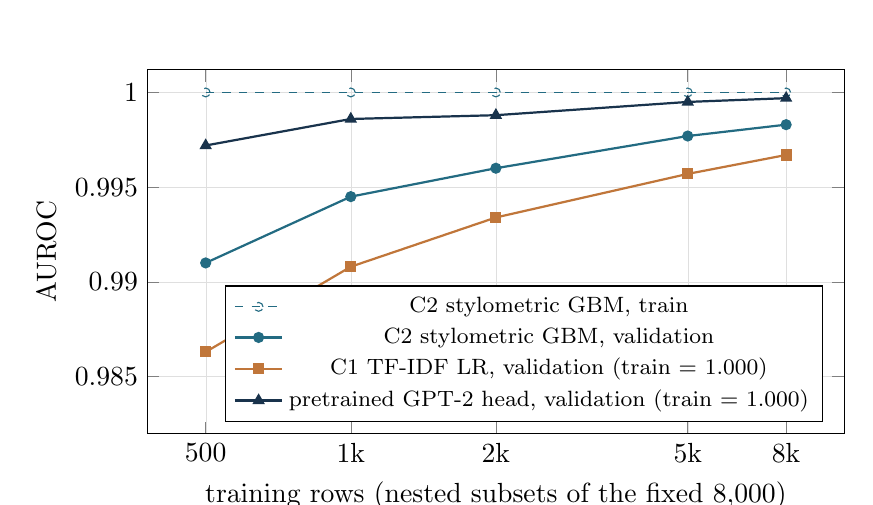
\begin{tikzpicture}
\begin{axis}[width=0.86\linewidth, height=6.2cm, xmode=log, log basis x=10,
  xtick={500,1000,2000,5000,8000}, xticklabels={500,1k,2k,5k,8k},
  xlabel={training rows (nested subsets of the fixed 8,000)}, ylabel={AUROC},
  ymin=0.982, ymax=1.0012, yticklabel style={/pgf/number format/fixed,/pgf/number format/precision=3},
  legend pos=south east, legend style={font=\footnotesize}, grid=both, grid style={line width=.1pt, draw=gray!25}]
\addplot[teal, dashed, mark=o, mark size=1.6pt] coordinates {
% <<gen curve:classical/results/experiments/learning_curve.csv:stylo_gbm:train_auroc
(500,1.0000) (1000,1.0000) (2000,1.0000) (5000,1.0000) (8000,1.0000)
% gen>>
};
\addlegendentry{C2 stylometric GBM, train}
\addplot[teal, thick, mark=*, mark size=1.6pt] coordinates {
% <<gen curve:classical/results/experiments/learning_curve.csv:stylo_gbm:val_auroc
(500,0.9910) (1000,0.9945) (2000,0.9960) (5000,0.9977) (8000,0.9983)
% gen>>
};
\addlegendentry{C2 stylometric GBM, validation}
\addplot[copper, thick, mark=square*, mark size=1.6pt] coordinates {
% <<gen curve:classical/results/experiments/learning_curve.csv:tfidf_lr:val_auroc
(500,0.9863) (1000,0.9908) (2000,0.9934) (5000,0.9957) (8000,0.9967)
% gen>>
};
\addlegendentry{C1 TF-IDF LR, validation (train = 1.000)}
\addplot[navy, thick, mark=triangle*, mark size=1.8pt] coordinates {
% <<gen curve:pretrained/results/learning_curve.csv:lm_gpt2:val_auroc
(500,0.9972) (1000,0.9986) (2000,0.9988) (5000,0.9995) (8000,0.9997)
% gen>>
};
\addlegendentry{pretrained GPT-2 head, validation (train = 1.000)}
\end{axis}
\end{tikzpicture}
\end{center}
\smallnote{Training AUROC is 1.000 at every size for all three models, so only C2's train curve is drawn.}
\question{Q2.3 [3 points].}{What does the curve suggest about overfitting, underfitting, and the value of more labeled examples?}
\textbf{No underfitting.} Every model separates its training rows perfectly (train AUROC 1.000) at every size, so training AUROC carries no information here; the validation curve is what matters.

\textbf{Overfitting shrinks with data but never disappears.} C2's train--validation gap falls from 0.009 at 500 rows to 0.0017 at 8,000. The gain per step shrinks from 0.0035 (500 to 1,000 rows) to 0.0006 (5,000 to 8,000), so the curve is flattening. C1 starts lower (0.986) and gains more from data (0.0044 for the first doubling, 0.0011 for the last step), as expected for a model with hundreds of thousands of sparse n-gram features. The pretrained GPT-2 head is at 0.997 with only 500 labels, because the LM supplies the representation.

\textbf{Value of more labels.} More labels \emph{of the same kind} would add little: at most a few thousandths, mainly for C1. The bigger gap is to test, whose domains and generators differ (C2 drops from 0.998 on validation to 0.960 on Kaggle). More \emph{diverse} labels, such as verse and new generators, would plausibly matter far more than more rows like these.

\section{Learning from unlabeled data (5 points)}
\textbf{Learning goal:} test whether the additional 3,000 unlabeled passages help.
\question{Q3.1 [2 points].}{Describe one method that uses \texttt{unlabeled.csv} (e.g., self-training, confidence-based pseudo-labeling, clustering, or feature learning). How did you prevent validation-label leakage?}
\textbf{Confidence-based self-training}, with hyperparameters held fixed:
\begin{enumerate}
\item Train on the 8,000 rows and score \texttt{unlabeled.csv}.
\item Label the 20\% highest-scored passages AI and the 20\% lowest human (1,200 pseudo-labels).
\item Retrain on the 8,000 rows plus these pseudo-labels.
\end{enumerate}
We ran 1 and 3 rounds (each round re-selects from the newest model) for C1, C2 and the pretrained GPT-2 head.

\textbf{Leakage control.} The validation rows are split off before anything is fit and scored once at the end. The pool is \texttt{unlabeled.csv} only (no test or validation text), and we checked that no unlabeled passage duplicates a validation passage (0 matches). The C3 tokenizer also uses \texttt{unlabeled.csv} text, never its labels (it has none).
\question{Q3.2 [2 points].}{Compare against a supervised baseline under the same held-out validation protocol.}
\begin{tabularx}{\linewidth}{@{}Yp{1.5in}@{}}\toprule Method & Validation AUROC \\ \midrule
% <<gen file:reports/tables/q32_semisup.tex
Supervised only (\texttt{lm\_gpt2}) & 0.99972 \\
Pseudo-labels, 1 round (\texttt{lm\_gpt2}) & 0.99972 \\
Pseudo-labels, 3 rounds (\texttt{lm\_gpt2}) & 0.99974 \\
\midrule
Supervised only (\texttt{tfidf\_lr}) & 0.99670 \\
Self-training, 1 round (\texttt{tfidf\_lr}) & 0.99659 \\
Self-training, 3 rounds (\texttt{tfidf\_lr}) & 0.99657 \\
Supervised only (\texttt{stylo\_gbm}) & 0.99831 \\
Self-training, 1 round (\texttt{stylo\_gbm}) & 0.99829 \\
Self-training, 3 rounds (\texttt{stylo\_gbm}) & 0.99835 \\
% gen>>
\bottomrule\end{tabularx}
\question{Q3.3 [1 point].}{Did it help? Give a concrete, evidence-based explanation (including possible noise in pseudo-labels).}
\textbf{No.} Every change is within $\pm$0.00013, below what 2,000 validation rows resolve.

\textbf{Why: the pseudo-labels carry no new information.} The passages confident enough to be selected are ones the model already gets right. For C2, every selected passage scored at least 0.99996 (AI) or at most 0.0001 (human); for C1, at least 0.974 or at most 0.033. Any wrong pseudo-labels are reinforced rather than corrected. The problem is uninformative pseudo-labels, not noisy ones.

\textbf{The pool also does not cover the shift.} \texttt{unlabeled.csv} has 1.2\% verse-like passages, like train (1.6\%), while test has 16.6\%. So it cannot teach what test needs.

\section{Generalization and error analysis (20 points)}
\textbf{Learning goal:} characterize how well the selected model generalizes and where it fails. Use \textbf{labeled validation data}; hidden test labels and hidden domain/generator information are unavailable.

\question{Q4.1 [5 points].}{Compare training and validation AUROC for your final selected model. Is there a gap? What explanations are plausible?}
\textbf{Blend A:} training AUROC 1.00000, validation 0.99987, a gap of only 0.0001. At a 0.5 threshold it misclassifies 9 of 2,000 validation passages (1 false positive, 8 false negatives). The gap is small because most of the representation comes from pretrained models: the frozen LMs never saw our labels, and the fine-tuned encoders start from general-purpose weights. Validation is also drawn from the same distribution as training. For comparison, the from-scratch C2 has a gap of 0.0017 (1.00000 against 0.99831), ordinary overfitting of 800 boosted trees.

\textbf{The gap that matters is to test:} 0.99987 on validation against 0.98810 public. Test has unseen generators and far more verse (16.6\% against 1.6\% of train), which validation cannot show. The shift hurts from-scratch models more: C2 falls from 0.99831 to 0.95995, and C3 from 0.98590 to 0.90826.

\question{Q4.2 [5 points].}{Evaluate performance over at least three text-length bins (define the bins), or another observable subgroup available in your data. Explain why you chose the grouping.}
\begin{tabularx}{\linewidth}{@{}Yrr@{}}\toprule Subgroup / bin (blend A, final model) & Count & Validation AUROC \\ \midrule
% <<gen file:pretrained/reports/tables/q42_subgroups.tex
$<$150 words (word count; 234 AI) & 380 & 1.00000 \\
150-250 words (word count; 444 AI) & 1049 & 0.99991 \\
$>$250 words (word count; 322 AI) & 571 & 0.99980 \\
prose (line structure; 804 AI) & 1400 & 0.99989 \\
short lines (lists, recipes) (line structure; 192 AI) & 575 & 0.99997 \\
verse (line structure; 4 AI) & 25 & 1.00000 \\
% gen>>
\midrule
\multicolumn{3}{@{}l}{\textit{C2 (from-scratch stylometric GBM), same rows}} \\
% <<gen file:classical/reports/tables/q42_subgroups.tex
$<$150 words (word count; 234 AI) & 380 & 0.99927 \\
150-250 words (word count; 444 AI) & 1049 & 0.99916 \\
$>$250 words (word count; 322 AI) & 571 & 0.99674 \\
prose (line structure; 804 AI) & 1400 & 0.99845 \\
short lines (lists, recipes) (line structure; 192 AI) & 575 & 0.99740 \\
verse (line structure; 4 AI) & 25 & 1.00000 \\
% gen>>
\bottomrule\end{tabularx}

\textbf{Groupings.}
\begin{itemize}
\item Word-count bins ($<$150, 150--250, $>$250 words): per-word rates and averaged LM statistics are noisier for short passages.
\item Line structure: verse ($\ge$4 lines, median $\le$10 words per line, no digits), short-line lists or recipes, and prose. Test is 16.6\% verse, and layout drives our stylometric model.
\end{itemize}

\textbf{Observed.} Blend A is at or above 0.9998 in every group. C2 is weakest on long passages (0.9967) and short-line lists (0.9974). Verse scores perfectly, but on only 25 rows (4 AI), so it is not informative. That is itself a finding: the subgroup that matters most for test is almost absent from the labelled data.

\question{Q4.3 [5 points].}{Analyze at least \textbf{five false positives and five false negatives} from your held-out validation set. Provide example IDs, predicted probabilities, and short failure hypotheses. Do not paste full passages unless essential.}

\textit{Blend A (our final pretrained model): its one false positive, its four highest-scored humans below 0.5 (near misses), and its five most confident false negatives.}

{\small\begin{tabularx}{\linewidth}{@{}p{0.45in}p{0.82in}p{0.42in}Y@{}}\toprule ID & Error type & P(AI) & Possible reason \\ \midrule
% <<gen file:pretrained/reports/tables/q43_errors.tex
\mbox{2696} & FP & 0.557 & Run-on, repetitive predictive-text-style ramble with no punctuation, whole phrases repeated; the GPT-2 token-stats-only member ranks it 0.93, the others 0.49-0.56 - repetitive low-perplexity text looks like small-model AI output. \\
\mbox{6067} & FP (near miss) & 0.497 & Near miss (P=0.497, below 0.5): student essay on information overload with a tidy argument structure (also a stylo\_gbm FP); hypothesis: essay register is predictable. \\
\mbox{9388} & FP (near miss) & 0.495 & Near miss (P=0.495): Wikipedia bio of composer Bright Sheng with a long list of orchestras; list-like encyclopedic prose is predictable. \\
\mbox{961} & FP (near miss) & 0.495 & Near miss (P=0.495): polished, upbeat movie review in clean paragraphs (also a stylo\_gbm FP); hypothesis: fluent and tidy, so few human-style irregularities. \\
\mbox{7384} & FP (near miss) & 0.491 & Near miss (P=0.491): short, informal movie review with run-on sentences; hypothesis: generic review phrasing is low-surprise for the LMs. \\
\mbox{5498} & FN & 0.427 & AI lasagna recipe with one ingredient per line and no blank lines (also a stylo\_gbm FN); ModernBERT ranks it 0.03 - hypothesis: the layout of human-scraped recipes reads as human. \\
\mbox{5603} & FN & 0.480 & AI casual first-person forum post about a game (also a stylo\_gbm FN); RoBERTa ranks it 0.20 - hypothesis: informal register and few formatting cues read as human. \\
\mbox{6331} & FN & 0.486 & AI bread recipe with ingredient lines and self-correcting notes ('it was my error to add...'); the token-stats-only member ranks it 0.17 - hypothesis: messy, human-like asides and recipe layout. \\
\mbox{3938} & FN & 0.489 & AI wiki-style article (View Askew universe) with long lists of film titles; every member near 0.5 - proper-noun lists look human to token statistics. \\
\mbox{3340} & FN & 0.490 & AI first-person forum post about feeding a cat, with curly apostrophes and cut off mid-question; RoBERTa ranks it 0.33 - hypothesis: informal advice-seeking register reads as human. \\
% gen>>
\bottomrule\end{tabularx}}

\needspace{14\baselineskip}\textit{C2 (from-scratch stylometric GBM), same validation rows: its five most confident errors of each type.}

{\small\begin{tabularx}{\linewidth}{@{}p{0.45in}p{0.82in}p{0.42in}Y@{}}\toprule ID & Error type & P(AI) & Possible reason \\ \midrule
% <<gen file:classical/reports/tables/q43_errors.tex
\mbox{9403} & FP & 0.954 & Encyclopedic physics abstract (semiconductor luminescence equations): long, uniform, formal sentences and no first person; hypothesis: formal expository register looks like AI style. \\
\mbox{961} & FP & 0.875 & Polished, upbeat movie review in clean paragraphs with few errors (one typo, 'throughly'); hypothesis: fluent and tidy, so few human-style irregularities. \\
\mbox{921} & FP & 0.859 & Wikipedia-style definition of interactionism with parentheticals and long sentences; same pattern as 9403. \\
\mbox{2696} & FP & 0.833 & Run-on, repetitive predictive-text-style ramble ('I hope to hear from you soon' twice); hypothesis: high repetition matches small-model AI text in train. \\
\mbox{6067} & FP & 0.647 & Formal student essay on information overload; tidy argument structure, moderate score (0.65); hypothesis: essay register. \\
\mbox{5498} & FN & 0.000 & AI lasagna recipe with an ingredient list one item per line and no blank lines; hypothesis: matches the line layout of human-scraped recipes, so line-structure features vote human. \\
\mbox{5316} & FN & 0.001 & Fluent biography of Hideki Tojo with invented facts (PM until 1997); hypothesis: wiki-bio register with no AI formatting cues - style features cannot check facts. \\
\mbox{7049} & FN & 0.002 & Spelt-dough recipe with bullet glyphs and 'o' sub-bullets, scraped-web layout; hypothesis: formatting mimics human scraped text. \\
\mbox{1602} & FN & 0.002 & Wiki-bio with a hatnote ('This article is about...') and [1] citation markers; hypothesis: copies human Wikipedia scraping artefacts that the model treats as human. \\
\mbox{5603} & FN & 0.006 & Casual first-person forum post about a game; hypothesis: informal register and few formatting cues read as human. \\
% gen>>
\bottomrule\end{tabularx}}
\smallnote{Threshold 0.5. A false positive is human text predicted AI; a false negative is AI text predicted human. Blend A makes only 1 false positive (and 8 false negatives) at 0.5, so its four highest-scored humans below 0.5 are added as near misses; the table shows its five most confident false negatives. To give more than five genuine false positives, the second table lists the five most confident errors of each type of C2, which makes 7 false positives and 19 false negatives on the same rows. For blend A, P(AI) is the weighted mean member percentile.}

\question{Q4.4 [5 points].}{What recurring failure patterns did you identify, and how might you address one of them? Distinguish observed patterns from speculation.}
\textit{Observed.}
\begin{enumerate}
\item \textbf{Blend A's errors are disagreements, not confident mistakes.} Every blend A error scores between 0.43 and 0.56, and most come from one member family dissenting: on 2696 the GPT-2 token-statistics-only head gives 0.93 while the others sit near 0.5; on 5498 ModernBERT gives 0.03; on 5603 RoBERTa gives 0.20.
\item \textbf{False negatives copy scraped-web layout or informal registers.} Recipes with one ingredient per line, a wiki-style list of film titles, casual first-person forum posts: formats and registers that train associates with human text.
\item \textbf{False positives are predictable human prose:} a repetitive ramble, and near misses that are a tidy essay, an encyclopedia bio and two generic movie reviews. C2's false positives are the same kind (a physics abstract, a definition, a tidy essay).
\item \textbf{The same passages fail across model families.} 2696, 5498, 5603 and 7049 are errors of both blend A and C2, and three of C1's five lowest-scored AI passages (1602, 7049, 5498) are false negatives of blend A or C2. C1 itself makes 7 false positives and 50 false negatives at 0.5 (\texttt{classical/results/tfidf\_lr/val\_pred.csv}).
\end{enumerate}
\textit{Speculation.} The human training text was scraped, so its formatting artefacts became ``human'' cues that AI text in the same format exploits. Predictable human prose has the low perplexity that LM features associate with AI.

\textit{A fix to test.} Augment AI training passages with scraped-web formatting (citation markers, hard wraps, bullets), so formatting stops implying ``human''. Then measure the shared false negatives on validation and with topic-held-out CV. A related shortcut, line length, is the one we did fix (Q5).

\newpage
\section{Open-ended improvements and insights (15 points)}
\textbf{Learning goal:} propose and test one improvement beyond the required baseline comparisons. This can be simple: a targeted feature change, alternate regularization scheme, ensemble, different representation, augmentation, or training approach. Sophistication alone does not earn credit.

\question{Q5.1 [3 points].}{What specific question or hypothesis motivated your improvement? What weakness or opportunity did you observe?}
\textbf{Weakness.} Validation was saturated: every reasonable model scored 0.98 or more, the top dozen within 0.0005. Yet our first from-scratch uploads fell sharply on Kaggle: C1 0.963 $\to$ 0.886 and C3 0.985 $\to$ 0.832. Test differs from train: it has unseen domains and generators, and 16.6\% verse against 1.6\%.

\textbf{Hypothesis.} The first versions rely on shortcuts that hold only inside train's topics: topic words for C1, line length for C3. (1) A validation scheme that holds out whole \emph{topics} of \texttt{train.csv} will expose the drop without any test labels or extra data, and (2) representations that remove those shortcuts will score higher on it and on Kaggle.

\question{Q5.2 [4 points].}{What exactly did you change? Describe the baseline, the new approach and what you held fixed for a fair comparison.}
\textbf{Topic-held-out CV} (\texttt{classical/train.py --cv topic}). K-means ($k=10$) on word TF-IDF of the 8,000 training rows only, seed 20261023; GroupKFold(5) holds out whole clusters (news; personal writing; reviews + recipes + biographies; baking + computer vision; science + cooking). Every fold keeps both classes.

\textbf{Baselines.} C1 v1 (word 1--2 + in-word character 2--5 TF-IDF); C3 v1 (raw text).

\textbf{Changes.}
\begin{itemize}
\item C1 adds raw-text character n-grams (layout visible) and word n-grams over text-distorted input \cite{stamatatos2017}, which masks every word outside the $k$ most frequent training words.
\item C3 joins single line breaks, so line length is no longer visible; blank lines stay.
\end{itemize}
\textbf{Selection.} The candidates (30 for C1, 11 for C3: distortion size, crops, dropout, depth) and the rule were committed before any run: highest mean topic-held-out AUROC, ties within one fold s.d.\ go to the simplest. Winners: C1 v3 (raw char + distorted, $k=100$, $C=4$) and C3 v3 (lines joined). v2 was an intermediate version of each.

\textbf{Held fixed.} Training rows, validation split, architectures, seeds, and hyperparameter choice inside the training rows only. Each new version was uploaded once.

\question{Q5.3 [4 points].}{What were the measured results?}
{\small\begin{tabularx}{\linewidth}{@{}Yrrrr@{}}\toprule Configuration & Val. AUROC & Runtime & Topic-held-out CV & Kaggle public \\ \midrule
% <<gen file:classical/reports/tables/q53_versions.tex
C1 v1: word + in-word char TF-IDF & 0.96256 & 16 s & 0.9134 $\pm$ 0.0340 & 0.88583 \\
C1 v2: + raw char, distorted (k=300), C=64 & 0.99678 & 23 s & 0.9875 $\pm$ 0.0083 & 0.96374 \\
C1 v3: + raw char, distorted (k=100), C=4 & 0.99670 & 25 s & 0.9869 $\pm$ 0.0095 & 0.95849 \\
C3 v1: raw text & 0.98500 & 38 s & 0.9047 $\pm$ 0.0699 & 0.83201 \\
C3 v2: lines joined, distorted (k=300) & 0.98903 & 32 s & 0.9725 $\pm$ 0.0067 & 0.91502 \\
C3 v3: lines joined & 0.98590 & 34 s & 0.9759 $\pm$ 0.0032 & 0.90826 \\
% gen>>
\bottomrule\end{tabularx}}

\textbf{Per held-out topic} (AUROC on each fold's held-out clusters; columns C1 v1/v2/v3, C3 v1/v2/v3):

{\small\begin{tabularx}{\linewidth}{@{}>{\RaggedRight}Yrrrrrrr@{}}\toprule Held-out topics (rows) & AI & C1 v1 & C1 v2 & C1 v3 & C3 v1 & C3 v2 & C3 v3 \\ \midrule
% <<gen file:classical/reports/tables/q53_topics.tex
1: said year (1,903) & 0.52 & 0.8652 & 0.9817 & 0.9794 & 0.8733 & 0.9750 & 0.9742 \\
2: like just (1,424) & 0.50 & 0.9103 & 0.9780 & 0.9762 & 0.9459 & 0.9689 & 0.9750 \\
3: movie film (474); chopped cup (107); born university (940) & 0.51 & 0.8891 & 0.9833 & 0.9825 & 0.9554 & 0.9822 & 0.9822 \\
4: dough flour (128); segmentation image (895); sugar cup (504) & 0.49 & 0.9510 & 0.9997 & 0.9999 & 0.9676 & 0.9740 & 0.9744 \\
5: study results (869); pepper heat (756) & 0.47 & 0.9515 & 0.9945 & 0.9963 & 0.7813 & 0.9622 & 0.9739 \\
\midrule
Mean & & 0.9134 & 0.9875 & 0.9869 & 0.9047 & 0.9725 & 0.9759 \\
S.d. & & 0.0340 & 0.0083 & 0.0095 & 0.0699 & 0.0067 & 0.0032 \\
% gen>>
\bottomrule\end{tabularx}}
\smallnote{Topic-CV values come from the design-selection runs (\texttt{classical/results/selection/}), where v1 and v2 are candidates too. ``AI'' is the AI share of the held-out rows. C3 trains on a GPU and is not bit-reproducible.}

\question{Q5.4 [4 points].}{What did you learn? Did the results support the hypothesis? What limits the conclusion, and what would you try next?}
\textbf{Supported.} Holding out topics reproduces what Kaggle showed: C1 v1 falls from 0.963 on validation to 0.913 on held-out topics (0.865 on news) and C3 v1 to 0.905 (0.781 on science and cooking), while C2, built on style features, stays at 0.995. The causes are visible per fold:
\begin{itemize}
\item \textbf{C1 relied on topic.} Raw character n-grams alone barely help on held-out topics (0.934); the distorted view, which removes topic words, lifts C1 to 0.987 and the news fold from 0.865 to 0.979. On Kaggle the change took C1 from 0.886 to 0.964 (v2).
\item \textbf{C3 learned ``short lines = AI''.} In train, human passages have long lines and AI passages short ones. Joining single line breaks removes that cue: held-out-topic AUROC rises from 0.905 to 0.976 and its spread across topics falls from 0.070 to 0.003. On Kaggle v2 went from 0.832 to 0.915.
\end{itemize}
Topic-held-out CV also set blend A's weights (Q1.4), where ordinary CV was saturated; it does not show that A beats B, because A was fit to that same score and the gap is within fold-to-fold noise.

\textbf{Lesson.} Formatting is usually real signal (removing layout features costs C2 0.011 on validation), but a model with no hand-made features can latch onto a single cue, and that shortcut must be removed. A validation scheme that mimics the shift, built from the training data alone, is enough to see it.

\textbf{Limits.} Topic clusters only approximate test's shift: they hold out domains, not generators, and train has almost no verse, so no fold resembles test's poems. Fold estimates are noisy (s.d.\ up to 0.01), which is why many C1 variants tie. Topic CV separates large effects (v1 against later versions) but not small ones: it put C1 v3 level with v2 and C3 v3 slightly above v2, while on the public leaderboard both v3s came in slightly lower (0.95849 against 0.96374, 0.90826 against 0.91502), differences near the leaderboard's own noise.

\textbf{Next.} Test the scraped-web augmentation (Q4.4); hold out generators as well as topics, if generator identity could be inferred without labels; pretrain C3 self-supervised from scratch on train plus unlabeled text.

\section{Code submission, reproducibility and AI assistance (10 points)}
\textbf{Submission format:} Submit a \textbf{GitHub PR URL} against the course repository. We will inspect the final code and its development history, not just the final snapshot. Do not squash away meaningful intermediate commits before review. Template \href{https://github.com/sekhari/human-or-ai-submissions}{here}.

\question{Q6.1 [5 points].}{Provide the PR URL, the entrypoint for training/evaluation, and the command used to generate \texttt{submission.csv}. State dependencies and random seeds.}
\textbf{PR:} \url{https://github.com/sekhari/human-or-ai-submissions/pull/25}

\textbf{Code:} \texttt{submissions/group-number-31/}. Its \texttt{README.md} covers setup and every command, and \texttt{MODELS.md} gives each submitted model's full pipeline.

\textbf{Final Kaggle selections:} blend A (\hf{pretrained/kaggle_submissions/final_A_topic_greedy.csv}) and C2 (\hf{classical/kaggle_submissions/final_D_stylo_gbm.csv}). Their private scores are revealed only after this report is due, so the report gives validation and public scores.

\textbf{Entry points}, run from that folder:
\begin{itemize}
\item \texttt{train.py}: train on the 8,000 rows and score the fixed 2,000, or \texttt{--final} to refit on 10,000 and write the Kaggle file.
\item \texttt{predict.py}: writes \texttt{submission.csv}.
\end{itemize}
{\footnotesize\begin{verbatim}
python common/make_split.py              # re-create + check the validation split
python predict.py --model blend_a --committed --out submission.csv
                                         # final file, exactly as uploaded
python predict.py --model blend_a --out submission.csv
                                         # re-predict from the saved runs (GPU)
python classical/select_design.py --model tfidf_lr --jobs 8
                                         # C1 design choice, topic-held-out CV
python train.py --model stylo_gbm        # C2: inner-CV search, fit 8k, score 2k
python train.py --model stylo_gbm --final
                                         # refit on 10k -> Kaggle file D
python predict.py --model stylo_gbm --out submission.csv
\end{verbatim}}
\textbf{Environment.} Python 3.11, the \texttt{cs-aml} conda environment (\texttt{pretrained/environment.yml}); \texttt{pip install -r requirements.txt} (numpy, pandas, scikit-learn, LightGBM, tokenizers, PyTorch, Hugging Face Transformers \cite{hftransformers}). The classical track runs on a laptop CPU. The pretrained track needs a 12 GB GPU and, for an RTX 50-series card, PyTorch built with CUDA 12.8+. Kaggle CSVs are not committed; pass \texttt{--data-dir} or set \texttt{HOA\_DATA\_DIR}.

\textbf{Seeds.} 20261023 for the split, all CV folds and every fixed-split experiment; the 5-fold runs behind the pretrained uploads used seed 42.

\textbf{Reproduction.} \texttt{predict.py} reproduces the committed classical files exactly (maximum difference 0) and blend B's file exactly (\texttt{pretrained/results/reproduction.csv}). Blends with fine-tuned members (A, C) re-predict with bf16 GPU noise; \texttt{make\_submission.py} prints the Spearman correlation to the committed file ($\ge$ 0.9999 when we ran it; this check is not stored in a results file).

\question{Q6.2 [3 points].}{Give two or three examples of changes you made during development. Link to relevant commits or PR discussion and briefly explain what the experiments taught you.}
\begin{itemize}
\item \commit{b91274d976dbae2b0b80a898386aa3d1770b8af8}{b91274d} $\to$ \commit{a23916e774ca31506d07339682d50c33eb477051}{a23916e}, \commit{6232de40d79fc3460035074d42be4c1bab261acc}{6232de4}: after C1 and C3 fell on Kaggle, we added topic-held-out CV and ran the design selection on it, which chose C1's and C3's final designs (rule in \hf{classical/configs/selection/}, results in \hf{classical/results/selection/}). \emph{Lesson:} when validation and the leaderboard disagree, make validation harder in the way test is harder, instead of tuning on the leaderboard, and decide the rule before seeing the results.
\item \commit{1fc181fef044ef79830a9a0db09f32bc305f38e0}{1fc181f}: a 35-job benchmark saturated CV (0.990--0.999), so blend weights could not be chosen on it; blend A's members and weights were then chosen by the same topic-held-out scheme (\hf{pretrained/results/blend_selection/}). \emph{Lesson:} saturated CV cannot choose between strong models.
\item \commit{6fb8406709d375571d760b4d23b11a131c61c44e}{6fb8406}, \commit{3754f3b7f2d07855ff6e01a9ef753e7f575d4698}{3754f3b}: removing C2's layout features cost 0.011 AUROC, and debiasing hurt the pretrained models too. \emph{Lesson:} formatting is real signal, so we kept it everywhere except the one model it misled.
\end{itemize}

\question{Q6.3 [2 points].}{How did you use AI tools (such as Claude, ChatGPT or Copilot) for code, debugging, analysis or writing? What did you verify or modify yourself?}
\textbf{Our decisions.} We decided the overall structure (two tracks on one fixed validation split), the model architectures, the candidate models and which analyses to run.

\textbf{Claude Code's role.} Claude Code (Anthropic) mainly wrote the code to those specifications and executed the experiments on our machines. It also helped draft report text, which we edited.

\textbf{What we verified and changed.}
\begin{itemize}
\item We read the data ourselves (verse, recipes, scraped-web layout, blank-line habits) and changed the pipelines along the way to match what we saw.
\item We checked every local score against the Kaggle score. When they disagreed (C1 and C3), we had the cause investigated and changed the models accordingly.
\item We ran everything in one conda environment after finding that a different interpreter silently replaced LightGBM with another booster.
\item We made every Kaggle upload and checked that every number in this report comes from committed results files.
\end{itemize}

\textbf{Rules followed, specifically.}
\begin{itemize}
\item \textbf{Supervised labels come only from \texttt{train.csv}.} Every model, in both tracks, is fit on \texttt{train.csv} rows: 8,000 for validation experiments, all 10,000 for the Kaggle files. \texttt{unlabeled.csv} is used without labels, for C3's tokenizer and the self-training experiment (Q3), where pseudo-labels come from our own model.
\item \textbf{No externally sourced labelled data.} Training, validation and every model choice behind the final submissions use \texttt{train.csv} labels only: hyperparameters by inner CV, designs and blend weights by topic-held-out CV on the same rows. No external LLM API was used anywhere; test passages were scored only by our own models.
\item \textbf{No hidden labels.} We did not search for or use test labels, generator names or domain information from any source. The only feedback from Kaggle was the public score of each upload. Every upload is listed in Appendix B; each new version was uploaded once and was not tuned against the leaderboard.
\item \textbf{Validation was not used for tuning the from-scratch models.} Their 2,000 validation rows are in no CV fold and were used only to report the chosen settings. The blends' weights were chosen on topic-held-out out-of-fold predictions over all 10,000 \texttt{train.csv} rows, which include the validation rows (see the validation protocol in Section 1).
\item \textbf{All pretrained weights are disclosed} in Appendix A, including the models we tried but did not submit. The from-scratch models (C1--C3) use no pretrained weights.
\end{itemize}

\textbf{AI policy.} You may use AI assistants for coding, debugging, explanations, brainstorming, and editing. We expect each team to exercise its own judgment, run experiments, check outputs, and understand its submitted approach. Sending the entire assignment to an AI tool and submitting its unverified output without meaningful involvement does not satisfy the objectives of this project. We will use the PR history, reproducible experiments and report together as evidence of engagement. \emph{Commit counts and the presence of AI-generated code are not themselves grading criteria.} Do not fabricate results or retrieve hidden test labels.


\section*{Final submission checklist}
\begin{itemize}[label=$\square$]
\item Final probabilities submitted to Kaggle for every \texttt{test.csv} ID.
\item Completed report, with all required answers, tables, figures and sources, submitted as PDF.
\item GitHub PR linked on the report title page and in the course submission portal.
\item Code and dependencies recreate final predictions (within reasonable numerical tolerance).
\item Relevant experiments and seed/configuration details are recorded.
\item AI-use disclosure is complete; hidden labels were not retrieved externally.
\end{itemize}

\appendix
\section*{Appendix A. Pretrained models in the submitted blends}
All checkpoints come from the Hugging Face Hub. The from-scratch models (C1--C3, files D--F) use no pretrained weights.

{\small\begin{longtable}{@{}p{2.2in}rp{2.35in}p{0.8in}@{}}
\caption{The pretrained checkpoints inside blends A--C (current versions), and how each is used.}\label{tab:pretrained}\\
\toprule Checkpoint (Hugging Face) & Params & How we used it & In blends \\ \midrule\endfirsthead
\toprule Checkpoint (Hugging Face) & Params & How we used it & In blends \\ \midrule\endhead
\multicolumn{4}{@{}l}{\textit{Frozen language models: token statistics as features for a LightGBM head (weights never updated)}} \\
\hf{openai-community/gpt2} \cite{gpt2} & 124M & per-token log-prob, rank, entropy (15 stats) & A, B, C \\
\hf{openai-community/gpt2-medium} \cite{gpt2} & 355M & same statistics, larger LM & A, B, C \\
\hf{Qwen/Qwen2.5-0.5B} + \hf{-Instruct} \cite{qwen25} & 0.5B & Binoculars observer/performer pair \cite{binoculars}: perplexity, cross-perplexity, Binoculars score & A, B, C \\
\hf{Qwen/Qwen2.5-1.5B} + \hf{-Instruct} \cite{qwen25} & 1.5B & same, larger pair & B, C \\
\midrule
\multicolumn{4}{@{}l}{\textit{Encoders fine-tuned end to end as classifiers (5-fold; test score = mean of the fold models)}} \\
\hf{distilbert/distilroberta-base} \cite{distilbert} & 82M & fine-tuned classifier & A, C \\
\hf{answerdotai/ModernBERT-base} \cite{modernbert} & 149M & fine-tuned classifier & A \\
\hf{FacebookAI/roberta-base} \cite{roberta} & 125M & fine-tuned classifier & A \\
\bottomrule
\end{longtable}}

\textbf{Earlier versions and models tried during development.} Blend A v1 also used DeBERTa-v3-large \cite{debertav3} and the RoBERTa-large GPT-2-output detector \cite{solaiman2019}. Tried, not submitted: DeBERTa-v3-base/small, ELECTRA-base \cite{electra}, the RoBERTa-base GPT-2-output detector, and BGE \cite{bge} and E5 \cite{e5} sentence embeddings.

\section*{Appendix B. Kaggle submissions}
Every file we uploaded, in upload order. A new version of a model replaces its file under the same letter (Q1.4, Q5); earlier versions are marked v1/v2 and stay in the repository's history. Validation = the fixed 2,000 rows. Private scores were not revealed before this report was due, so that column is empty. The full testing history of every model we validated, including those never uploaded, is in \texttt{SUBMISSIONS.md} in the repository.

{\small\begin{tabularx}{\linewidth}{@{}lYrrrl@{}}\toprule
File & Model & Val. AUROC & Public & Private & Commit \\ \midrule
% <<gen file:reports/tables/kaggle_uploads.tex
A (v1) & Blend A, v1: 7 models, weights 3,3,2,1,1,1,1 & 0.99990 & 0.99161 & -- & \href{https://github.com/ZhenmanShen/human-or-ai-submissions/commit/c7c1e3e5c379f092b31d1ef745dbf2900d052f03}{\texttt{c7c1e3e}} \\
B & Blend B: 4 frozen-LM heads, equal weights & 0.99985 & 0.98848 & -- & \href{https://github.com/ZhenmanShen/human-or-ai-submissions/commit/c7c1e3e5c379f092b31d1ef745dbf2900d052f03}{\texttt{c7c1e3e}} \\
C (v1) & Blend C, v1: blend B + RoBERTa-base & 0.99987 & 0.98845 & -- & \href{https://github.com/ZhenmanShen/human-or-ai-submissions/commit/c7c1e3e5c379f092b31d1ef745dbf2900d052f03}{\texttt{c7c1e3e}} \\
D & C2 stylometric GBM & 0.99831 & 0.95995 & -- & \href{https://github.com/ZhenmanShen/human-or-ai-submissions/commit/08cde9152812e9dc60a72a394012065253065643}{\texttt{08cde91}} \\
E (v1) & C1 TF-IDF + LR, first version & 0.96256 & 0.88583 & -- & \href{https://github.com/ZhenmanShen/human-or-ai-submissions/commit/d0cfc4c8c92c432b47f372ca6f7cf3db06f780c2}{\texttt{d0cfc4c}} \\
F (v1) & C3 Transformer, first version & 0.98500 & 0.83201 & -- & \href{https://github.com/ZhenmanShen/human-or-ai-submissions/commit/a0679175ad4b0fa0a04df438aad48b956f1b26f5}{\texttt{a067917}} \\
E (v2) & C1 TF-IDF + LR, v2 (k=300, C=64) & 0.99678 & 0.96374 & -- & \href{https://github.com/ZhenmanShen/human-or-ai-submissions/commit/05e04170434cf5204e08a0a844ad4e91aaf9045f}{\texttt{05e0417}} \\
F (v2) & C3 Transformer, v2 (lines joined, distorted) & 0.98903 & 0.91502 & -- & \href{https://github.com/ZhenmanShen/human-or-ai-submissions/commit/05e04170434cf5204e08a0a844ad4e91aaf9045f}{\texttt{05e0417}} \\
A & Blend A: 7 models, greedy weights on topic-held-out CV & 0.99987 & 0.98810 & -- & \href{https://github.com/ZhenmanShen/human-or-ai-submissions/commit/1274dc4394837261c3a9ba9633361b205a38b576}{\texttt{1274dc4}} \\
C & Blend C: blend B + DistilRoBERTa & 0.99994 & 0.98724 & -- & \href{https://github.com/ZhenmanShen/human-or-ai-submissions/commit/1274dc4394837261c3a9ba9633361b205a38b576}{\texttt{1274dc4}} \\
E & C1 TF-IDF + LR, v3 (chosen by topic-held-out CV) & 0.99670 & 0.95849 & -- & \href{https://github.com/ZhenmanShen/human-or-ai-submissions/commit/a23916e774ca31506d07339682d50c33eb477051}{\texttt{a23916e}} \\
F & C3 Transformer, v3 (chosen by topic-held-out CV) & 0.98590 & 0.90826 & -- & \href{https://github.com/ZhenmanShen/human-or-ai-submissions/commit/6232de40d79fc3460035074d42be4c1bab261acc}{\texttt{6232de4}} \\
% gen>>
\bottomrule\end{tabularx}}

{\small
\begin{thebibliography}{99}\setlength{\itemsep}{1pt}
\bibitem{gpt2} A.~Radford, J.~Wu, R.~Child, D.~Luan, D.~Amodei, I.~Sutskever. Language Models are Unsupervised Multitask Learners. OpenAI technical report, 2019.
\bibitem{qwen25} Qwen Team. Qwen2.5 Technical Report. arXiv:2412.15115, 2024.
\bibitem{binoculars} A.~Hans et al. Spotting LLMs With Binoculars: Zero-Shot Detection of Machine-Generated Text. ICML 2024; arXiv:2401.12070.
\bibitem{roberta} Y.~Liu et al. RoBERTa: A Robustly Optimized BERT Pretraining Approach. arXiv:1907.11692, 2019.
\bibitem{debertav3} P.~He, J.~Gao, W.~Chen. DeBERTaV3: Improving DeBERTa using ELECTRA-Style Pre-Training with Gradient-Disentangled Embedding Sharing. ICLR 2023; arXiv:2111.09543.
\bibitem{solaiman2019} I.~Solaiman et al. Release Strategies and the Social Impacts of Language Models. arXiv:1908.09203, 2019 (the GPT-2 output detectors).
\bibitem{distilbert} V.~Sanh, L.~Debut, J.~Chaumond, T.~Wolf. DistilBERT, a distilled version of BERT: smaller, faster, cheaper and lighter. arXiv:1910.01108, 2019 (DistilRoBERTa follows the same recipe).
\bibitem{modernbert} B.~Warner et al. Smarter, Better, Faster, Longer: A Modern Bidirectional Encoder for Fast, Memory Efficient, and Long Context Finetuning and Inference (ModernBERT). arXiv:2412.13663, 2024.
\bibitem{electra} K.~Clark, M.-T.~Luong, Q.~V.~Le, C.~D.~Manning. ELECTRA: Pre-training Text Encoders as Discriminators Rather Than Generators. ICLR 2020.
\bibitem{bge} S.~Xiao et al. C-Pack: Packed Resources For General Chinese Embeddings (BGE models). SIGIR 2024; arXiv:2309.07597.
\bibitem{e5} L.~Wang et al. Text Embeddings by Weakly-Supervised Contrastive Pre-training (E5). arXiv:2212.03533, 2022.
\bibitem{hftransformers} T.~Wolf et al. Transformers: State-of-the-Art Natural Language Processing. EMNLP 2020 (System Demonstrations).
\bibitem{lightgbm} G.~Ke et al. LightGBM: A Highly Efficient Gradient Boosting Decision Tree. NeurIPS 2017.
\bibitem{sklearn} F.~Pedregosa et al. Scikit-learn: Machine Learning in Python. JMLR 12, 2011.
\bibitem{ma2023} Y.~Ma et al. AI vs.\ Human -- Differentiation Analysis of Scientific Content Generation. arXiv:2301.10416, 2023.
\bibitem{stamatatos2017} E.~Stamatatos. Authorship Attribution Using Text Distortion. EACL 2017.
\bibitem{bpe} R.~Sennrich, B.~Haddow, A.~Birch. Neural Machine Translation of Rare Words with Subword Units. ACL 2016.
\bibitem{transformer} A.~Vaswani et al. Attention Is All You Need. NeurIPS 2017.
\bibitem{caruana2004} R.~Caruana, A.~Niculescu-Mizil, G.~Crew, A.~Ksikes. Ensemble Selection from Libraries of Models. ICML 2004.
\end{thebibliography}}

\end{document}
